 %!TEX TS-program = lualatex
%!TEX encoding = UTF-8 Unicode

\documentclass[12pt, hidelinks]{exam}

%\printanswers

\usepackage{fontspec}
\setmainfont[Ligatures={TeX}, BoldFont={* Bold}, ItalicFont={* Italic}, BoldItalicFont={* BoldItalic}, Numbers={OldStyle}]{Linux Libertine O}
\setsansfont[Scale=MatchLowercase,Ligatures=TeX]{Linux Biolinum O}
%\setmonofont[Scale=MatchLowercase]{Inconsolatazi4}
\usepackage{microtype}

\usepackage{xcolor}
\usepackage{graphicx}
	\graphicspath{{/Users/goby/Pictures/teach/163/lab/}
	{img/}} % set of paths to search for images

\usepackage{geometry}
\geometry{letterpaper, left=1.5in, bottom=1in}                   
%\geometry{landscape}                % Activate for for rotated page geometry
\usepackage[parfill]{parskip}    % Activate to begin paragraphs with an empty line rather than an indent
\usepackage{amssymb, amsmath}
\usepackage{mathtools}
	\everymath{\displaystyle}



% To define fonts for particular uses within a document. For example, 
% This sets the Libertine font to use tabular number format for tables.
 %\newfontfamily{\tablenumbers}[Numbers={Monospaced}]{Linux Libertine O}
% \newfontfamily{\libertinedisplay}{Linux Libertine Display O}

\usepackage{booktabs}
\usepackage{multicol}
\usepackage[normalem]{ulem}

\usepackage{longtable}
%\usepackage{siunitx}
\usepackage{array}
\newcolumntype{L}[1]{>{\raggedright\let\newline\\\arraybackslash\hspace{0pt}}p{#1}}
\newcolumntype{C}[1]{>{\centering\let\newline\\\arraybackslash\hspace{0pt}}p{#1}}
\newcolumntype{R}[1]{>{\raggedleft\let\newline\\\arraybackslash\hspace{0pt}}p{#1}}

\usepackage{tikz}
\usetikzlibrary{shapes, arrows, arrows.meta}

\usepackage{forest}
\forestset{
	every leaf node/.style={
		if n children=0{#1}{}
	},
	every tree node/.style={
		if n children=0{}{#1}
	},
	mytree/.style={
		for tree={
			edge path={
				\noexpand\path [draw, very thick, \forestoption{edge}] (!u.parent anchor) |- (.child anchor)\forestoption{edge label};
			},
			every tree node={draw=none,inner sep=0, outer sep=0, minimum size=0},
			every leaf node/.style={align=left},
			grow=east,
			parent anchor=south, 
			child anchor=west,
			anchor=west,
			l sep=5mm,
			s sep=3mm,
			draw=none,
			if n children=0{tier=word}{}
		}
	}
}


\tikzstyle{decision} = [chamfered rectangle, chamfered rectangle xsep=2cm, draw, text width=10em, text centered]
\tikzstyle{block} = [rectangle, draw, text width=10em, text centered, rounded corners, minimum height=4em]
\tikzstyle{result} = [draw, ellipse, minimum width=2cm]
%\tikzstyle{line} = [draw, -latex', thick]

\tikzstyle{line} = [draw, arrows={-Stealth[length=3mm]}]


\usepackage{enumitem}
%\setenumerate{label=\Alph.}
\setlist{leftmargin=*}
\setlist[1]{labelindent=\parindent}
\setlist[enumerate]{label=\textsc{\alph*}.}
\setlist[itemize]{label=\color{gray}\textbullet}

\usepackage{hyperref}
%\usepackage{placeins} %PRovides \FloatBarrier to flush all floats before a certain point.
\usepackage{hanging}

\usepackage[sc]{titlesec}

%% Commands for Exam class
\renewcommand{\solutiontitle}{\noindent}
\unframedsolutions
\SolutionEmphasis{\bfseries}

% Shifts margins left. Question numbers appear in margin.
% This allows "fullwidth" to left align with text that is outside 
% if the questions environment.
\renewcommand{\questionshook}{%
	\setlength{\leftmargin}{-\leftskip}%
}

%\renewcommand{\partshook}{%
%	\setlength{\leftmargin}{-\leftskip}%
%}

%Change \half command from 1/2 to .5
%\renewcommand*\half{.5}

\pagestyle{headandfoot}
\firstpageheader{\textsc{bi}\,063 Evolution and Ecology}{}{\ifprintanswers\textbf{KEY}\else Name: \enspace \makebox[2.5in]{\hrulefill}\fi}
\runningheader{}{}{\footnotesize{pg. \thepage}}
\footer{}{}{}
\runningheadrule

\newcommand*\AnswerBox[2]{%
    \parbox[t][#1]{0.92\textwidth}{%
    \begin{solution}#2\end{solution}}
    \vspace{\stretch{1}}
}

\newenvironment{AnswerPage}[1]
    {\begin{minipage}[t][#1]{0.92\textwidth}%
    \begin{solution}}
    {\end{solution}\end{minipage}
    \vspace{\stretch{1}}}

\newlength{\basespace}
\setlength{\basespace}{5\baselineskip}


%\usepackage{mdframed}
%\mdfsetup{%
%	innerleftmargin=0pt,%
%	innerrightmargin=0pt,
%	innertopmargin=0pt,
%	innerbottommargin=0pt,
%	hidealllines=true
%}%end mdfsetup


\begin{document}

\subsection*{Using homology for phylogenetic hypotheses}

You have learned how to use the presence and absence of shared
characters to construct phylogenetic trees. You have also learned that \emph{homologies}
are similar characters shared between organisms due to common ancestry and that
\emph{analogies} are similar characters shared between unrelated organisms, 
often because the similarity serves similar functions in similar environments.

Only homologous characters can be used to build phylogenetic trees because 
homologies are evidence of common ancestry. Analogous characters do not provide 
evidence of ancestry so they cannot be used to build phylogenetic trees. For example, 
the following data for four species uses one homology (symmetry) and two analogies (wings, 
streamlining). The wings provide lift so that robins and dragonflies can fly. The streamlined
body of dolphins and tunas reduce drag when they swim through dense water.


\bigskip

\begin{center}

	\begin{tabular}{lC{0.8in}C{0.6in}C{0.8in}}
		\toprule
		Species	& Bilateral Symmetry	&	Wings	&	Streamlined Body \tabularnewline
		\midrule
		Dolphin 	&	1						&	0					&	1	\tabularnewline 
		Tuna Fish	&	1						&	0					&	1	\tabularnewline
		Robin		&	1						&	1					&	0	\tabularnewline
		Dragonfly	&	1						&	1					&	0	\tabularnewline
		\bottomrule
	\end{tabular}

\bigskip

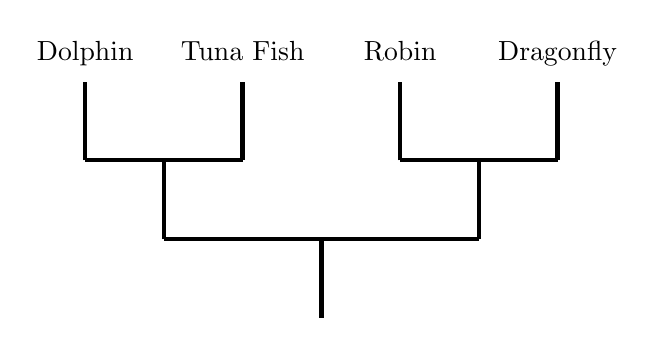
\begin{tikzpicture}
	[branch/.style={ultra thick}]
	
	\draw [branch] (0,0) -- (0,1);
	\draw [branch] (-2,1) -- (2,1);
	\draw [branch] (-2,1) -- (-2,2);
	\draw [branch] (2,1) -- (2,2);
	\draw [branch] (-3,2) -- (-1,2);
	\draw [branch] (1,2) -- (3,2);
	\draw [branch] (-3,2) -- (-3, 3) node [above] {\strut Dolphin};
	\draw [branch] (-1,2) -- (-1, 3) node [above] {\strut Tuna Fish};
	\draw [branch] (1,2) -- (1, 3) node [above] {\strut Robin};
	\draw [branch] (3,2) -- (3, 3) node [above] {\strut Dragonfly};

\end{tikzpicture}

\end{center}

\bigskip

The result is an incorrect phylogeny. For example, dolphins and robins
 are endothermic (“warm-blooded”), and have amniotic eggs and four appendages
 (tetrapods). Tunas share the presence of a notochord and vertebrae with the 
 dolphin and robin. These characters are all homologies. If the above phylogeny was
 correct, then the dragonfly should also have those characters but it does not.

A phylogenetic tree based only on homologies strongly (next page) supports a closer relationship 
for robin, tuna, and dolphin, which better reflects the scientific understanding of 
evolutionary history.

\begin{center}
	\begin{tabular}{lC{0.8in}C{0.7in}C{0.8in}}
		\toprule
		Species	& Bilateral Symmetry	&	Has Vertebrae	&	Amniotic Egg \tabularnewline
		\midrule
		Dolphin 	&	1						&	1					&	1	\tabularnewline 
		Tuna Fish	&	1						&	1					&	0	\tabularnewline
		Robin		&	1						&	1					&	1	\tabularnewline
		Dragonfly	&	1						&	0					&	0	\tabularnewline
		\bottomrule
	\end{tabular}

\bigskip

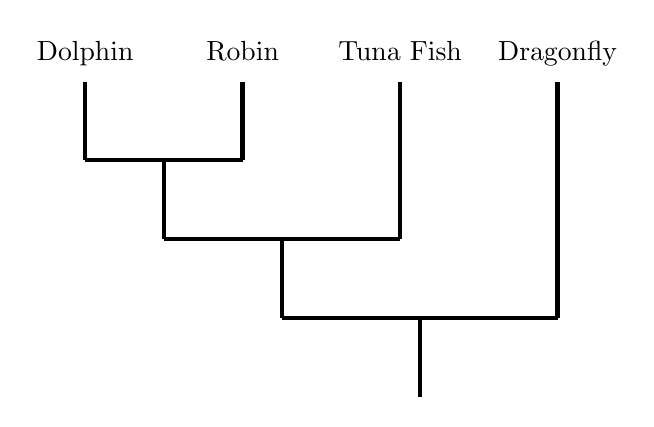
\begin{tikzpicture}
	[branch/.style={ultra thick}]
	
	\draw [branch] (0.25,0) -- (0.25,1);
	\draw [branch] (-1.5,1) -- (2,1);
	\draw [branch] (2,1) -- (2,4) node [above] {\strut Dragonfly};
	\draw [branch] (-1.5,1) -- (-1.5,2);
	\draw [branch] (-3,2) -- (0,2);
	\draw [branch] (0,2) -- (0, 4) node [above] {\strut Tuna Fish};
	\draw [branch] (-3,2) -- (-3,3);
	\draw [branch] (-4,3) -- (-2,3);
	\draw [branch] (-4,3) -- (-4, 4) node [above] {\strut Dolphin};
	\draw [branch] (-2,3) -- (-2, 4) node [above] {\strut Robin};

\end{tikzpicture}

\end{center}

\bigskip

Recall that phylogenetic trees are \emph{hypotheses} about relationships,
and that hypotheses make predictions. Therefore, phylogenetic trees 
\emph{predict} the presence of homologies among organisms. This phylogeny
predicts that a homology should be shared between a sea star and a clam that
is not shared by the fungus and oak tree. In turn, the fungus and
oak tree should share a homology that is not shared with the clam and sea star. 
The tree also predicts that all four organisms should share at least one
homology.

\bigskip

\begin{center}

  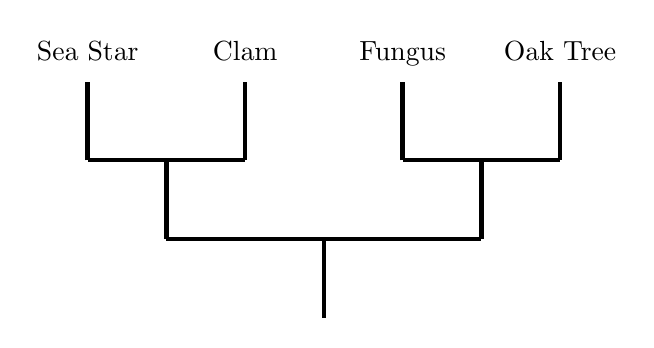
\begin{tikzpicture}
  	[branch/.style={ultra thick}]
  	
  	\draw [branch] (0,0) -- (0,1);
  	\draw [branch] (-2,1) -- (2,1);
  	\draw [branch] (-2,1) -- (-2,2);
  	\draw [branch] (2,1) -- (2,2);
  	\draw [branch] (-3,2) -- (-1,2);
  	\draw [branch] (1,2) -- (3,2);
  	\draw [branch] (-3,2) -- (-3, 3) node [above] {\strut Sea Star};
  	\draw [branch] (-1,2) -- (-1, 3) node [above] {\strut Clam};
  	\draw [branch] (1,2) -- (1, 3) node [above] {\strut Fungus};
  	\draw [branch] (3,2) -- (3, 3) node [above] {\strut Oak Tree};
  
  \end{tikzpicture}

\end{center}

\bigskip

What about analogies? Does the tree above predict that sea star and clam will
share analogies? How about between fungus and oak tree? 
Analogies could exist between almost any two
organisms. Analogy does not depend on them being related but instead that they
share a structure that has a similar function. The phylogeny itself does not 
make any predictions about analogies---the predictions are just about relationships, 
and not about the functions of structures in the various organisms.

\subsubsection*{Homology versus analogy}

So, homologies can be used to make phylogenetic trees but analogies cannot. 
Phylogenetic trees can predict the presence of homologies but not analogies. 
\emph{How then can you distinguish between homology and analogy?} If you know the 
common ancestor, you can see if the structure is present in the species and the
ancestor. If the structure is present in the ancestor, then the similarity must be due
to homology. If the structure is absent, then the similarity in the descendants must be due to analogy.

Usually, though, you will be looking at similar characters in living organisms to test
hypotheses about their ancestry, without knowing anything about the ancestor.  When 
you see similar structures shared among two or more species, there are two
testable explanations for it. They are

\begin{enumerate}
	\item \emph{homology:} the structures are similar because the species
inherited the similarity from a common ancestor, and

	\item \emph{analogy:} the similarity is necessary for a particular function.\footnote{The similarity
could be due solely to chance, but this would be \emph{very}
unlikely.} 
\end{enumerate}

\bigskip

This flow chart shows how to decide whether a structural similarity 
is a homology or analogy. 

\begin{center}

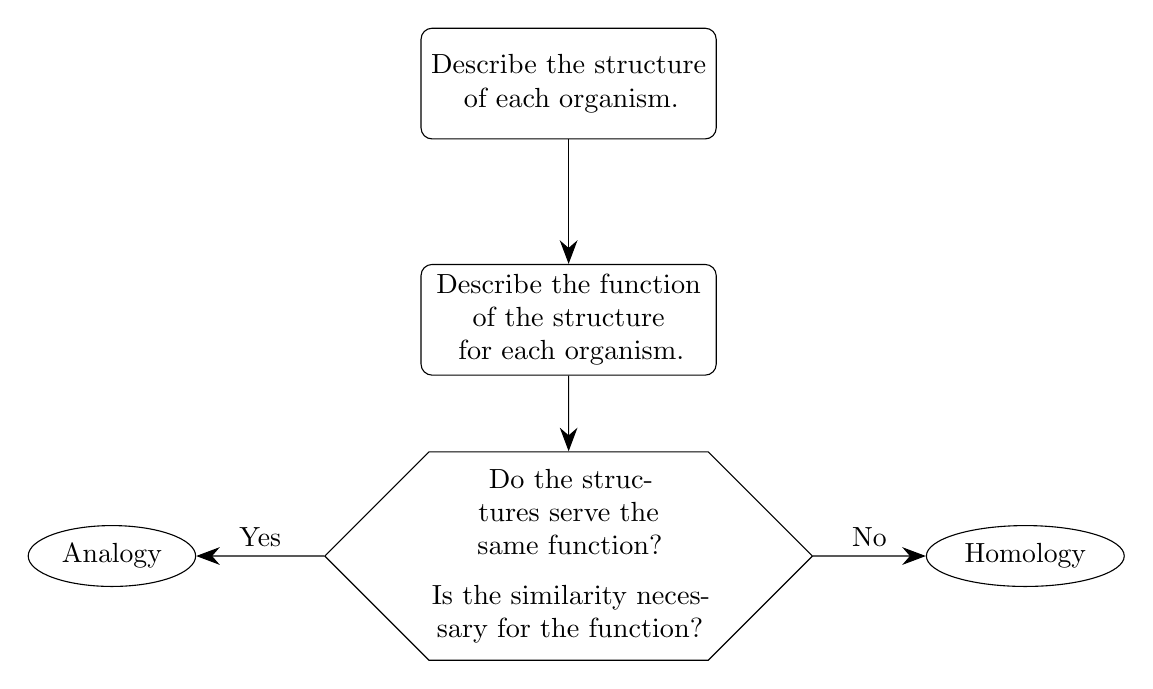
\begin{tikzpicture}[node distance = 3cm]

	\node [block] (structure) {Describe the structure of each organism.};
	
	\node [block, below of=structure] (function) {Describe the function of the structure for each organism.};

	\node [decision, below of=function] (decide) {Do the structures serve the same function?\\ \medskip
	Is the similarity necessary for the function?};
	
	\node [result, left of=decide, node distance=5.8cm] (analogy) {Analogy};
	
	\node [result, right of=decide, node distance=5.8cm] (homology) {Homology};
	
	\path [line] (structure) -- (function);
	\path [line] (function) -> (decide);
	\path [line] (decide) ->  node [above] {Yes}  (analogy);
	\path [line] (decide) -- node [above] {No} (homology);
	
\end{tikzpicture}

\end{center}

\bigskip

You first describe the structure you are comparing
between two organisms. Descriptions should contain enough detail to make
a valid comparison. For example, if you are comparing wings of a robin and a 
dragonfly, you should state that they are long, broad, thin, and very light weight.
You next describe the function of the structures. The wings both serve the
function of providing lift for the organisms to fly. 

You then decide if the structural similarity is necessary to serve the specific function. 
If the answer is “Yes,” then you conclude the structures are analogous. If the answer is
”No,” then you conclude the structures are homologous. For lift, it is necessary to have
structures that are long and broad for surface area to provide lift. Thin structures can
move through air easily, reducing drag. Light weight structures move easily and
save energy. Thus, a reasonable conclusion is that the similar wing structure of
a robin and a dragonfly are necessary for the function and therefore analogies.

\textsc{Important:} You \emph{must} understand how to compare structure and function
using this flow chart. \emph{You may be asked to draw and apply the flow chart on an exam.}

\subsubsection*{Homology or analogy? Comparing skeletons}

For the rest of this lab, you will determine whether several structural similarities
shared among vertebrate organisms are homologous or analogous, using the flow chart.

\begin{questions}

\question
Compare the clavicle (``collar bone'') of a macaque to the clavicle of a cat. In these animals, the clavicle is located between the top of the sternum and the shoulder.

%\begin{longtable}[c]{@{}rll@{}}
%  \toprule
%  Macaque &
%  \includegraphics[width=0.3\textwidth]{07_clavicle_macaque1}	&
%  \includegraphics[width=0.3\textwidth]{07_clavicle_macaque2}	\tabularnewline
%  \midrule
%  Cat &
%  \includegraphics[width=0.3\textwidth]{07_clavicle_cat2}	&
%  \includegraphics[width=0.3\textwidth]{07_clavicle_cat1}	\tabularnewline
%  \bottomrule
%\end{longtable}

In the macaque (and most other vertebrates), the clavicle is the only bone connection between
the forelimb and the trunk of the body. Note how it makes contact with
the sternum at one end and the shoulder blade at the other. 

In the cat, the clavicle does \emph{not} connect between the shoulder blade and the trunk of
the body (it didn't have those metal springs in there when it was
alive). %The arrow in the right photo of a cat's shoulder shows
The cat's clavicleis approximately the same shape as the
the macaque and is located in the same area of the body. (It also forms
the same way during embryonic development.) The cat's clavicle doesn't touch
any other bone or cartilage in the cat; it is embedded in a muscle on the
chest. The clavicle's position here is slightly off to the side from where it's
found in the living cat because it has been attached with a wire to the
humerus.

\begin{parts}

\part Describe their structural similarity. What is similar about their 
structure, that is, their shape, location, composition, and other features?

	\AnswerBox{4\baselineskip}{\emph{This question has no point value.}}

\part What is the function of the clavicle in each organism? For example, consider how monkeys like
the macaque climb trees, hanging from branches
and swinging. How would a bone connection between the arm and chest be
helpful? 
For the cat, what good is a tiny little bone that doesn't touch
any other bone?

macaque: \ifprintanswers{\textbf{\textit{This question has no point value.}}}\fi\\[3\baselineskip]

cat: \\[2\baselineskip]

\part Is the similarity you described above necessary in order to
serve the functions? Explain.

	\AnswerBox{4\baselineskip}{No. The clavicle serves the function of strengthening the shoulder girdle in the macaque (they will not say shoulder girdle). The clavicle does not serve a function in the cat.}

\part What do you conclude? Is the structural similarity you
described explained by homology or analogy?

	\AnswerBox{2\baselineskip}{Homology. The clavicle serves different functions between the two animals.}

\part If you concluded homology of the clavicle, do you think this
homology applies only to cats and macaques? What if we compared the
clavicle of the cat to the clavicle of a salamander, a turtle, or a pigeon? Would you conclude that the clavicle is a
homology or analogy? Explain.

	\AnswerBox{4\baselineskip}{Homology. In most vertebrates, the clavicle provides rigidity and support. But, not for the cat. If each vertebrate is compared to the cat, would conclude homology.}

\end{parts}

\newpage

\question
Consider the forelimb of the human and the cat. Each
has a first segment containing a single bone, the humerus, followed by a
second segment containing two bones, the radius and ulna. The structural similarity here is {the presence of two bones in the
second section of the forelimb of pigeon and human.}


%\begin{longtable}[c]{@{}L{2.5in}L{2.5in}l@{}}
%  \toprule
%  \centering \includegraphics[height=3cm]{07_radius_human1} &
%   \centering \includegraphics[height=3cm]{07_radius_human2}\tabularnewline
%   %
%  \centering \includegraphics[height=3cm]{07_radius_pigeon} &
%  \centering \includegraphics[height=3cm]{07_radius_human3}\tabularnewline
%  %
%  The pigeon's wing is folded. The joint between the humerus and
%  the radius and ulna (``elbow'') is along the back of the body. The ``hand'' of the pigeon
%  contains three digits, two of them mostly fused together. %
%  & %
%  The upper photo shows the radius
%  and ulna articulating with the wrist in the human arm. The lower photo shows the
%  human ulna (lower left) and radius (upper left) forming the elbow joint
%  with the humerus (right).\tabularnewline
%  \bottomrule
%\end{longtable}

\begin{parts}
	\part What is the function of the radius and ulna in each
animal? Hint: feel your own arm at the wrist and move your hand
various ways. Twist your wrist. What sort of motion do two bones allow?
Can cats make similar motions with their forelegs? Can a cat turn the pads of its paws upward like you can with your palm?

human: \ifprintanswers{\textbf{\textit{This question has no point value}}}\fi\\[2\baselineskip]

cat: \\[1\baselineskip]

\part Is the similarity (having two bones in the forearm)
necessary in order to serve the \emph{function(s)}? Explain.

	\AnswerBox{4\baselineskip}{No. The radius and ulna allows for rotation in human but not pigeon.}

\part What do you conclude? Is the structural similarity you
described explained by homology or analogy? Explain.

	\AnswerBox{4\baselineskip}{Homology. The radius and ulna serve different functions.}

\part If you concluded homology of the radius and ulna, do you
think this homology applies only to humans and cats? What if we
compared the radius and ulna of the human to the other vertebrate
organisms that have them, like salamanders, pigeons, or turtles? What might you conclude? Explain.

	\AnswerBox{2\baselineskip}{The radius and ulna are homologous among the vertebrates. In most cases, they do not allow rotation like humans.}
\end{parts}

%Now, consider a bison (buffalo). Like cattle, bison have hooves, and they
%support a great deal of weight on them. Their front hooves cannot rotate
%with respect to the rest of the limb (in fact, you can imagine that it
%might be pretty dangerous for the ``wrist'' of a bison to turn,
%considering the weight it supports).
%
%Below are two different hypotheses that include the bison. Based 
%on what you know of bison, and of the radius and ulna,
%what would each hypothesis \emph{predict} about the forelimb of
%the bison? Which hypothesis predicts that the bison would more
%likely have two bones in the second part of the forelimb, or only one?
%Give your answer and explain why that answer is the one predicted by
%each hypothesis.
%
%\begin{multicols}{2}
%
%	Hypothesis \textsc{a:} \medskip
%	
%	\includegraphics[width=0.9\columnwidth]{07_hypA}
%
%	\vspace*{0.5\baselineskip}
%	
%\columnbreak
%
%	Hypothesis \textsc{b:} \medskip
%	
%	\includegraphics[width=0.9\columnwidth]{07_hypB} 
%	
%	\vspace*{\baselineskip}
%
%\end{multicols}
%
%\question
%What does each hypothesis predict?
%
%\AnswerBox{5\baselineskip}{Hypothesis A predicts that the bison should not have the radius and ulna homology with any of the other organisms. Hypothesis B predicts that all of them should have the radius
%and ulna homology, including the bison.}
%
%Now go down to the student lounge (\textsc{mg} 127; turn right out the door, 
%the left, and halfway down the hall on the left) and have a look at the bison
%skeleton in the case. 
%
%Note that there are two bones in the second section 
%of the forelimb of the bison. Look carefully at the "wrist" joint; the two bones 
%(radius and ulna) are fused together there (the black vertical line is a wire holding the
%skeleton together). In fact, the bones are at least partially fused all
%along their length. They start out as two separate bones in the embryo,
%but fuse during development. By the time the bison is born, the two
%bones can't move separately from each other at all.

%\question
%What did you observe? Does this bison have a single bone, two clearly defined bones, or something else?
%
%\AnswerBox{5\baselineskip}{Two bones partially fused together.}
%
%\question
%Which hypothesis above was supported? Which was falsified? Explain why for each hypothesis.
%
%\AnswerBox{4\baselineskip}{Hypothesis \textsc{b} was supported. It predicted that the bison shares a common ancestor with the other organisms that have a radius and ulna. The bison has the \textsc{r\&u}, supporting the hypothesis of common ancestry. Hypothesis \textsc{a} predicted the bison did not have common ancestry with the other organisms so it should not have a homology with them. However, the \textsc{r\&u} appears to be a homology so the hypothesis was falsified.}

\newpage

\subsubsection*{Homology or analogy? Comparing vertebrate embryos}

Skeletal anatomy is just one type of evidence that can
be used to test for common ancestry. Another type of evidence is the 
embryo stage of vertebrates. Embryos have features that can
also be compared for homologies.
Here are some photos of vertebrate embryos. They have been scaled to
the same size, rotated to the same angle, converted to 
black and white, placed on dark backgrounds so that you can compare 
them easily. The photos were taken with different
photographic techniques, so that introduces some differences into their
overall appearance. They are not quite all at the same developmental
stage, but they are close.

\begin{longtable}[c]{@{}lll@{}}
\toprule
\includegraphics[height=5cm]{07_vert_embryo_A_chicken} 	&
\includegraphics[height=5cm]{07_vert_embryo_B_zebrafish}	&
\includegraphics[height=5cm]{07_vert_embryo_C_human}\\
A \ifprintanswers\textbf{\large Chicken}\fi & 
B \ifprintanswers\textbf{\large Zebrafish}\fi & 
C \ifprintanswers\textbf{\large Human}\fi  \\[4ex]
\midrule
\includegraphics[height=5cm]{07_vert_embryo_D_cat}	&
\includegraphics[height=5cm]{07_vert_embryo_E_salamander}	&
\includegraphics[height=5cm]{07_vert_embryo_F_turtle}\\
D \ifprintanswers\textbf{\large Cat}\fi &
E \ifprintanswers\textbf{\large Salamander}\fi 	&	
F \ifprintanswers\textbf{\large Turtle}\fi \\[4ex]
\bottomrule
\end{longtable}


\question
Can you identify the human? How about the
salamander, turtle, chicken, cat, and zebrafish? Place the names next to the appropriate letter. 

\AnswerBox{2\baselineskip}{Yes I can. See above.}

Embryos have many structures that have little or no
function during the embryo stage; they become useful after birth. As a result, 
the structures tend not to be modified much by natural selection. For example,
\emph{all of these embryos, including the human, have tails;} that is,
portions of the backbone that extend beyond the hind legs. You can see the tails 
in the photos on the previous page.

Now consider the following detailed drawings of nine vertebrate embryos.
The illustrated regions correspond to the head, throat and upper body.
In the throat region are \emph{pharyngeal arches}, indicated by the
bracket or arrows. These arches are found in all vertebrate embryos. 
In fishes, pharyngeal arches develop into the gills. In other animals, 
they develop into other structures in the throat region. Like the tail, the pharyngeal
arches do not have a function in the embryo.

\begin{center}
	\includegraphics[width=\textwidth]{07_vert_embryo_pharygeal_arches}
\end{center}

\question
Are the similarities of a tail and pharyngeal arches in these embryos due to homology or analogy? Explain.

\AnswerBox{3\baselineskip}{Homology. The tail and pharyngeal arches do not serve any function. Therefore,
the tail and pharyngeal arches are homologous among vertebrates.}

\question
The skeletal features and embryo evidence support common ancestry for these six organisms. 

\begin{multicols}{3}

	cat \\
%	bison \\
	fish \columnbreak
	
	human \\
	pigeon \columnbreak
	
	salamander \\
	turtle 
		
\end{multicols}

Make a phylogenetic tree for these six organisms based on evidence gathered so far. \emph{You may have been told not to have more than two branches coming from one node. It is \textsc{ok and necessary} to ignore that requirement for now.} Show your tree to your instructor for approval. Do not draw a tree based on what you \emph{think} are the relationships. Draw a tree using only the evidence gathered so far. (You can use the last page for practice.)

%\AnswerBox{0.45\textheight}{Tree goes here.}
\begin{AnswerPage}{0.45\textheight}

Something like: 

\begin{forest} mytree
	[[	
	[cat]
	[fish]
	[human]
	[pigeon]
	[turtle]
	[salamander]
	]]
\end{forest}

%\begin{center}
%	\begin{tikzpicture}
%		[branch/.style={thick}]
%		
%		\draw [branch] (0,0) -- (0,1);
%		\draw [branch] (0,1) -- (-3,4) node [above] {\strut cat};
%		\draw [branch] (0,1) -- (-2,4) node [above] {\strut fish};
%		\draw [branch] (0,1) -- (-0.75,4) node [above] {\strut human};
%		\draw [branch] (0,1) -- (0.75,4) node [above] {\strut pigeon};
%		\draw [branch] (0,1) -- (2,4) node [above] {\strut turtle};
%		\draw [branch] (0,1) -- (3,4) node [above right, xshift=-10pt] {\strut salamder};
%
%	\end{tikzpicture}
%\end{center}
\end{AnswerPage}

\end{questions}

The evidence so far supports common ancestry for these vertebrates but it cannot tell which of these six organisms might be most closely related. The next exercise will solve that problem.

\end{document}  